\documentclass[11pt, letterpaper]{article}
\usepackage{tabularx} % Advanced table configurations
\usepackage[utf8]{inputenc}
\textwidth 6.5in
\textheight 9in
\oddsidemargin 0in
\headheight 0in
\usepackage[english]{babel}
\usepackage[left=2.5cm,right=2.5cm,top=2cm,bottom=2cm]{geometry}
\usepackage{indentfirst}
\usepackage{graphicx}
\usepackage{float}
\usepackage[hidelinks]{hyperref}
\usepackage{mathtools}
\usepackage{preview}
\usepackage{enumitem}
\usepackage{subfiles}
\usepackage{import}
\usepackage{cancel}
\usepackage{amsmath}
\usepackage{tikz}
\usepackage{pifont}
\usepackage{relsize}
\usepackage{amssymb}
\usepackage{booktabs}
\usepackage{threeparttable}
\usepackage{caption}

%\def\input@path{{}}
%\def\input@path{{``C:/Users/Nicolás Urdaneta/Documents/GitHub/RDD/Tables/''}}
%\graphicspath{{``C:/Users/Nicolás Urdaneta/Documents/GitHub/RDD/''}}
\newcommand*{\commonpath}{C:/Users/Nicolás Urdaneta/Documents/GitHub/RDD}
\hypersetup{
    colorlinks=true,
}


\addto\captionsspanish{\renewcommand*\contentsname{Contenido}}

\title{\huge Fourth assignment}
\author{\LARGE Nicolás Urdaneta}
\date{June 13, 2020}

\setlength{\parindent}{0cm}
\begin{document}
\maketitle

\section*{Github repo and summary}

\begin{enumerate}
	\item {\itshape Download Hansen\_dwi.dta from github at the following address. \\
	\url{https://github.com/scunning1975/causal-inference-class/raw/master/hansen_dwi} \\
	Create a new github repo named ``RDD''.  Inside the RDD directory, put all the subdirectories we’ve discussed in class. Post the link to the repo so I can see it’s done as discussed.  Save the Hansen\_dwi.dta file into your new \/data subdirectory.  Note: The outcome variable is ``recidivism'' or ``recid'' which is measuring whether the person showed back up in the data within 4 months. } \\

	Here is the link to the repository:	\url{https://github.com/Nurdaneta/RDD}

	\item \textit{In the writing subdirectory, place your assignment.  For the first part, read Hansen’s paper in the \/articles directory of the main class github entitled ``Hansen AER''.  \textbf{Briefly summarize this paper}.  What is his question? What data does he use?  What is his research design, or “identification strategy”?  What are his conclusions? } \\

	Hansen (2015) is looking into the effect of being punished and sanctioned when driving under the influence of alcohol to test whether this might reduce drunk driving. To do answer his question, he looks for administrative data on all stops to test for people driving under influence (DUI) in the state of Washington from 1999 to 2007. He looks for people that in a window of up to four years after being stopped relapsed and was caught drunk driving again. \\

	He works on the fact that there is a threshold in blood alcohol content (BAC) from which punishment begins. If BAC is above 0.08 it is considered a DUI while if it is above 0.15 it is an aggravated DUI. This allows a regression discontinuity design around those two cutoffs. This particular identification strategy works very well as one may consider to be ``as good as random'' to be in either side of the cutoff by a small margin. \\

	He concludes that punishment reduces recidivism by about two percentage points, an effect close to 20\% of the average recidivism. And when testing for possible mechanisms, he provides evidence that is seems that deterrence from committing future infractions is the main source of his findings. As people that are being caught with DUI are punished and are most likely to avoid committing the crime again. Hansen suggests that to reduce recidivism it may me useful to reduce the cutoffs of DUI or increase the marginal penalty of commiting DUI. \\

\end{enumerate}


\section*{Replication}
\begin{enumerate}
	\setcounter{enumi}{2}
	\item \textit{In the United States, an officer can arrest a driver if  after giving them a blood alcohol content test they learn the driver had a BAC of 0.08 or higher.  We will only focus on the 0.08 BAC cutoff. We will be ignoring the 0.15 cutoff for all this analysis. Create a dummy equaling 1 if \textbf{bac1}$\geq$ 0.08 and 0 otherwise in your do file or R file.}

	\item \textit{The first thing to do in any RDD is look at the raw data and see if there’s any evidence for manipulation (``sorting on the running variable'').  If people were capable of manipulating their blood alcohol content (bac1), describe the test we would use to check for this.  Now evaluate whether you see this in these data?  Either recreate Figure 1 using the bac1 variable as your measure of blood alcohol content or use your own density test from software.  Do you find evidence for sorting on the running variable? } \\

	To test for manipulation we create a histogram and mark the cutoff point to see if there is an abrupt change in the distribution at the cutoff. Although it is actually hard to tell, there seems to be some small jump at the right side of the cutoff. This isn't a statistical test, the actual test is presented in Table 1 with the test proposed by Cattaneo et al. (2019) that takes on the McCrary test. This test is run with cutoffs at 0.04, 0.06 and the original 0.08 with the intention of running some placebo tests at other points to check that the 0.08 level creates an actual discontinuity. The results indicate that there is in fact a change in the density only at 0.08, resulting in manipulation. This differs from the test displayed by Hansen (2015) in which there seems to be no jump in the distribution, probably because he used the original McCrary test.  \\

	\begin{figure}[H]
		\centering
		\caption*{Figure 1: BAC Distribution}
		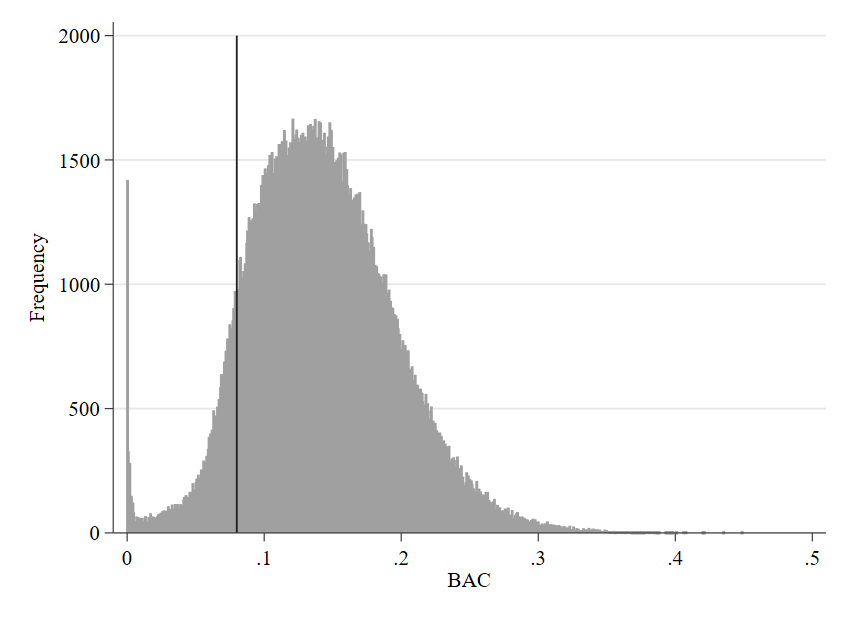
\includegraphics[scale=0.4]{\commonpath/Figures/Hist.png}
	\end{figure}

	\begin{table}[H]
		\centering
		\caption{McCrary test for manipulation from Cattaneo et al. (2019)}
		\begin{tabular}{cc}
		\toprule
		Cutoff tested & P-value \\ \hline
		0.04 & 0.668 \\
		0.06 & 0.995 \\
		0.08 & 0.028 \\ \hline \hline
		\end{tabular}
	\end{table}


	\item \textit{The second thing we need to do is check for covariate balance.  Recreate Table 2 but only white male, age and accident (acc) as dependent variables.  Use your equation (1) for this. Are the covariate balanced at the cutoff?  It’s okay if they are not exactly the same as Hansen’s.} \\

	Table 2 reports the covariate balance of male, age, race and accidents. The results indicate that there is no change in these variables at the cutoff as the coefficients are small and never significant. Which supports the continuity assumption in this research design. \\ 

	\begin{center}
\begin{table}[H] \centering
\captionsetup{justification=centering}
\caption{Regression Disctontinuity Estimates for the Effect \\ of Exceeding BAC Thresholds on Predetermined Characteristics}
\begin{threeparttable}
\begingroup
\setlength{\tabcolsep}{10pt}
\renewcommand{\arraystretch}{1.5}
 % Default value: 1
\begin{tabular}{l*{4}{c}}
\toprule
& \multicolumn{3}{>{\centering\arraybackslash}m{150pt}}{Driver demographic characteristics} & \\ \cline{2-4}
& Male & White & Age & Accident \\
Characteristics & (1) & (2) & (3) & (4) \\
\hline
DUI                 &       0.006   &       0.006   &      -0.140   &      -0.003   \\
                    &     (0.006)   &     (0.005)   &     (0.164)   &     (0.004)   \\
\\
Observations        &      89,967   &      89,967   &      89,967   &      89,967   \\
Mean (at 0.079)     &        0.80   &        0.86   &       33.62   &        0.10   \\
\hline \hline
\end{tabular}
\endgroup
\begin{tablenotes} \centering
\small
\item This table contains egression discontinuity based estimates of                   the effect of having BAC above the DUI threshold on recidivism.                   Panel A contains estimates with a bandwidth of 0.05 while Panel B                   has a bandwidth of 0.025, with all regressions utilizing a rectangular                   kernel for weighting.                    Robust standard errors. * p$<$0.10, ** p$<$0.05, *** p$<$0.01
\end{tablenotes}
\end{threeparttable}
\end{table}
\end{center}


	\item \textit{Recreate Figure 2 panel A-D. You can use the -cmogram- command in Stata to do this.  Fit both linear and quadratic with confidence intervals. Discuss what you find and compare it with Hansen’s paper.} \\

	Figures 2A and 2B show very similar results to those of Hansen and the ones presented in Table 2: there is no evidence of discontinuity in relevant observable covariates. Even though there might be non observable confounders that may cause a violation of continuity, the indication that these variables have no ``jumps'' is a good indication that there is no manipulation at the cutoff. This result holds both in the linear and quadratic specifications. \\

	\begin{figure}[H]
		\centering
		\caption*{Figure 2A: BAC and Characteristics. Linear polynomial}
		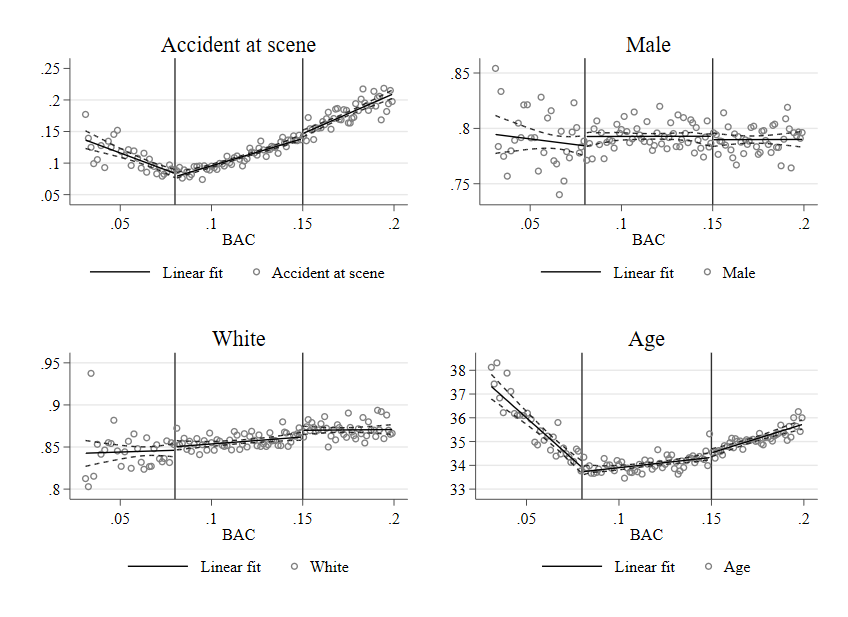
\includegraphics[scale=0.37]{\commonpath/Figures/Fig1a.png}
	\end{figure}
	\begin{figure}[H]
		\centering
		\caption*{Figure 2B: BAC and Characteristics. Linear polynomial}
		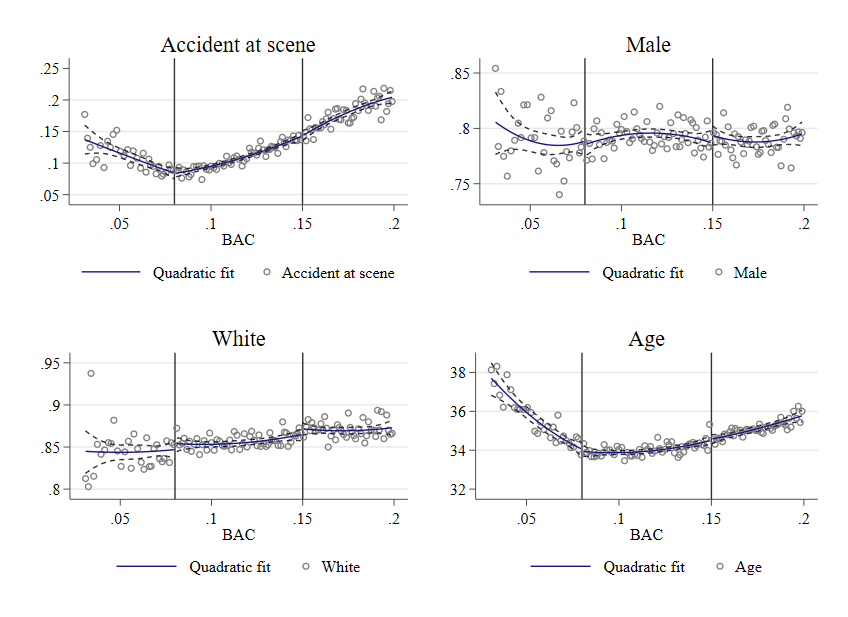
\includegraphics[scale=0.37]{\commonpath/Figures/Fig1b.png}
	\end{figure}
	\begin{tablenotes}
		\centering
		\small
		\item Confidence intervals at 95\%.
	\end{tablenotes}

	\item \textit{Estimate equation (1) with recidivism (recid) as the outcome.  This corresponds to Table 3 column 1, but since I am missing some of his variables, your sample size will be the entire dataset of 214,558.  Nevertheless, replicate Table 3, column 1, Panels A and B.  Note that these are local linear regressions and Panel A uses as its bandwidth 0.03 to 0.13.  But Panel B has a narrower bandwidth of 0.055 to 0.105.  Your table should have three columns and two A and B panels associated with the different bandwidths.:}
	\begin{enumerate}[label=(\alph*)]
		\item \textit{Column 1: control for the bac1 linearly}
		\item \textit{Column 2: interact bac1 with cutoff linearly}
		\item \textit{Column 3: interact bac1 with cutoff linearly and as a quadratic}
		\item \textit{For all analysis, use heteroskedastic robust standard errors.}
	\end{enumerate}

	Table 3 presents the results of the treatment of DUI at the discontinuity on recidivism. While the first column estimates a regression in which the polynomial is the same at both sides of the discontinuity, this coefficient shouldn't be the one to look. In fact, the coefficients of columns two and three allow the polynomial to be distinct at each side of the cutoff (linear in column two and quadratic in column three). The effect of being just above the cutoff leads to a reduction of 2 percentage points in recidivism (an effect of about 20\% of the average recidivism).  \\

	%PanelA
	\begin{center}
\begin{table}[H] \centering
\captionsetup{justification=centering}
\caption{Regression Disctontinuity Estimates for the Effect \\ of Exceeding BAC Thresholds on Recidivism}
\begin{threeparttable}
\begingroup
 % Default value: 1
\begin{tabular}{l*{3}{>{\centering\arraybackslash}m{3cm}}}
\toprule
& Linear BAC & Linear BAC with interaction & Quadratic BAC with interaction \\
 & (1) & (2) & (3) \\ \hline
Panel A. BAC $\in$ [0.03,0.013] & & & \\
DUI                 &      -0.027***&      -0.024***&      -0.014** \\
                    &     (0.004)   &     (0.004)   &     (0.006)   \\
\\
Observations        &      89,967   &      89,967   &      89,967   \\
Mean                &        0.12   &        0.12   &        0.12   \\

	%PanelB
	\\ 
Panel B. BAC $\in$ [0.055,0.105] & & & \\ 
DUI                 &      -0.022***&      -0.020***&      -0.014   \\
                    &     (0.006)   &     (0.006)   &     (0.008)   \\
\\
Observations        &      46,957   &      46,957   &      46,957   \\
Mean                &        0.12   &        0.12   &        0.12   \\
\hline \hline
\end{tabular}
\endgroup
\begin{tablenotes} \centering
\small
\item This table contains egression discontinuity based estimates of                   the effect of having BAC above the DUI threshold on recidivism.                   Panel A contains estimates with a bandwidth of 0.05 while Panel B                   has a bandwidth of 0.025, with all regressions utilizing a rectangular                   kernel for weighting. Controls include indicators for year, race,                    gender, and age of the offender (not county).                    Robust standard errors in parenthesis.                    * p$<$0.10, ** p$<$0.05, *** p$<$0.01
\end{tablenotes}
\end{threeparttable}
\end{table}
\end{center}


	\item \textit{Recreate the top panel of Figure 3 according to the following rule: }
	\begin{enumerate}[label=(\alph*)]
		\item \textit{Fit linear fit using only observations with less than 0.15 bac on the bac1}
		\item \textit{Fit quadratic fit using only observations with less than 0.15 bac on the bac1}
	\end{enumerate}

	Figure 3 presents the equivalent to the same figure from Hansen (2015). In it, it shows the effect on recidivism caused by the discontinuity in BAC that leads to the punishment. As it turns out, being caught with an alcohol level just above the threshold leads to a reduction in recidivism. Both the linear fit and quadratic fit are consistent to the findings of Table 3 in which there is a reduction in about two percentage points when being caught with an alcohol level above 0.08. \\

	\begin{figure}[H]
		\centering
		\caption*{Figure 3: BAC and Recidivism}
		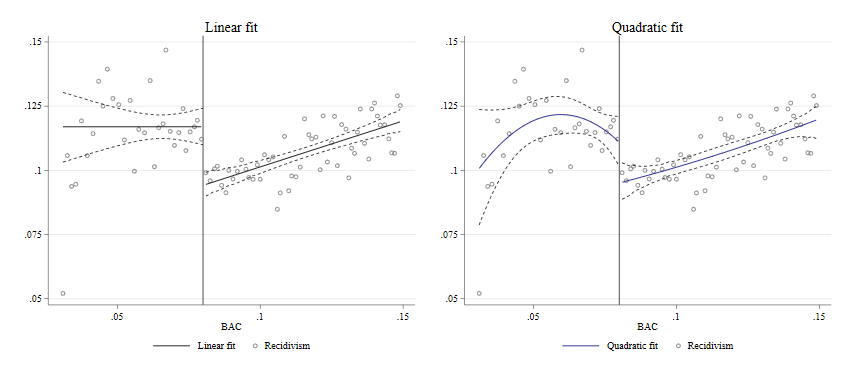
\includegraphics[width=1\textwidth]{\commonpath/Figures/Fig2.png}
	\end{figure}
	\begin{tablenotes}
		\centering
		\tiny
		\item Confidence intervals at 95\%.
	\end{tablenotes}

	\section*{References}
	Hansen, B. (2015). ``Punishment and Deterrence: Evidence from Drunk Driving.''
	\textit{American Economic Review}. 105(4): 1581–1617\\

	\noindent Cattaneo, M. D., Jansson, M., and Ma, X. (2017) ``rddensity: Manipulation
	Testing Based on Density Discontinuity.'' \textit{The Stata Journal}. ii: 1-24.


\end{enumerate}


\end{document}